\documentclass[11pt]{article}
\usepackage{geometry}
\usepackage{graphicx}
\usepackage{booktabs}
\usepackage{caption}
\usepackage{amsmath}
\usepackage{microtype}
\usepackage{subcaption}
\geometry{margin=1in}

\title{LLM Researcher Degrees of Freedom: Meta-Analysis of DACA Employment Replications}
\author{NHK Replications Project}
\date{\today}

\begin{document}
\maketitle

\section{Introduction}
This report summarizes Phase 4 of the NHK replications project, which adapts the ``many analysts'' framework of Huntington-Klein et al.\ to a stochastic LLM setting. Each LLM run is treated as an independent researcher who selects a specification for estimating the employment effect of DACA eligibility among Hispanic, foreign-born noncitizens. The meta-analysis characterizes the resulting distribution of estimates and documents how specification and implementation choices relate to the estimated effect sizes.

\section{Data and Methods}
The analysis uses \texttt{runs\_complete.csv}, which aggregates Phase 1 LLM specifications with Phase 2 execution results. In Phase 1, each LLM agent receives a standardized prompt to estimate the DACA employment effect and returns a structured specification: sample restrictions, outcome construction, treatment definition, and a model specification line. In Phase 2, each specification is executed against the ACS/IPUMS data in a clean run directory, and the resulting coefficient on the DACA eligibility indicator (or specified interaction) is recorded along with its standard error and sample size. We treat each successful execution as one ``researcher'' in the multiverse.

We restrict the sample to successful executions and drop runs with missing point estimates, standard errors, or sample sizes. To mitigate extreme artifacts from parsing or execution errors, we additionally trim observations with absolute point estimates greater than 1. All summary statistics, tables, and figures below are based on this filtered sample. Unless otherwise noted, all reported estimates use the LLM-chosen estimation method (e.g., OLS or WLS), weighting, and standard-error adjustment.

Point estimates refer to the coefficient on the DACA-eligibility indicator or interaction, as defined in each LLM-generated model specification. Standard errors are taken from the execution output and correspond to the estimation method and variance adjustment requested by the LLM. Sample sizes are the number of observations used in each executed specification.

\paragraph{Estimation pipeline.} Each run begins with the LLM-specified sample selection logic (e.g., age bounds, immigration timing, citizenship status, and year ranges) applied to the underlying microdata. The outcome variable is constructed exactly as specified by the LLM (typically employment or full-time employment indicators). The treatment variable encodes DACA eligibility using the LLM-provided rule, sometimes combined with timing indicators (e.g., post-2012 interactions). The model specification line is executed in Python, typically via \texttt{statsmodels} formula syntax, and can include linear terms, quadratic terms, categorical fixed effects ($C(\cdot)$), and interactions. If a weighting variable is supplied (most commonly \texttt{PERWT}), it is passed to the estimator. Variance adjustments such as heteroskedasticity-robust or clustered standard errors are applied using the estimator's covariance options. The resulting coefficient and its standard error are written to \texttt{results.json} and ingested into the meta-analysis.

\paragraph{Specification feature extraction.} For the method and controls tables, we parse each specification line to classify estimation method (OLS/WLS/other), weighting choice (PERWT/none/other), and variance adjustment (clustered/robust/other). Control-variable functional forms are inferred from the parsed formula: linear terms (e.g., \texttt{AGE}), quadratic terms (e.g., \texttt{I(AGE**2)}), and categorical fixed effects (e.g., \texttt{C(EDUC)}). These classifications allow us to summarize how specification components are associated with different estimated effects.

\section{Results}

\begin{table}[htbp]
\centering
\caption{Summary statistics for reported estimates}
\small
\resizebox{\textwidth}{!}{\begin{tabular}{@{}l r r r r r r r r@{}}
\toprule
Label & N & Mean & SD & Min & Pctl. 25 & Median & Pctl. 75 & Max \\
\midrule
Effect Size (unweighted) & 38 & 0.019 & 0.094 & -0.195 & -0.008 & 0.003 & 0.031 & 0.456 \\
Effect Size (weighted by inverse SE) & 38 & 0.021 & 0.076 & -0.195 & -0.006 & 0.003 & 0.031 & 0.456 \\
Standard Error & 38 & 0.007 & 0.009 & 0.000 & 0.004 & 0.005 & 0.007 & 0.054 \\
Sample Size & 38 & 180,775 & 148,116 & 6,780 & 61,288 & 123,602 & 258,390 & 530,881 \\
\bottomrule
\end{tabular}}
\caption*{\textbf{Notes:} The table reports distributional statistics for point estimates, standard errors, and sample sizes across all valid LLM-generated specifications. The inverse-SE weighted effect-size row uses weights $1/\max(SE, q_{0.25})$, where $q_{0.25}$ is the 25th percentile of $SE$, for the mean, SD, and percentiles; minimum and maximum are the sample extrema. Sample size statistics use the number of observations actually included in each executed model after the LLM-specified sample restrictions and data cleaning steps. Estimates with $|\hat{\beta}|>1$ are excluded by construction.}
\label{tab:summary}
\end{table}

\begin{figure}[htbp]
\centering
\begin{subfigure}[b]{0.48\textwidth}
    \centering
    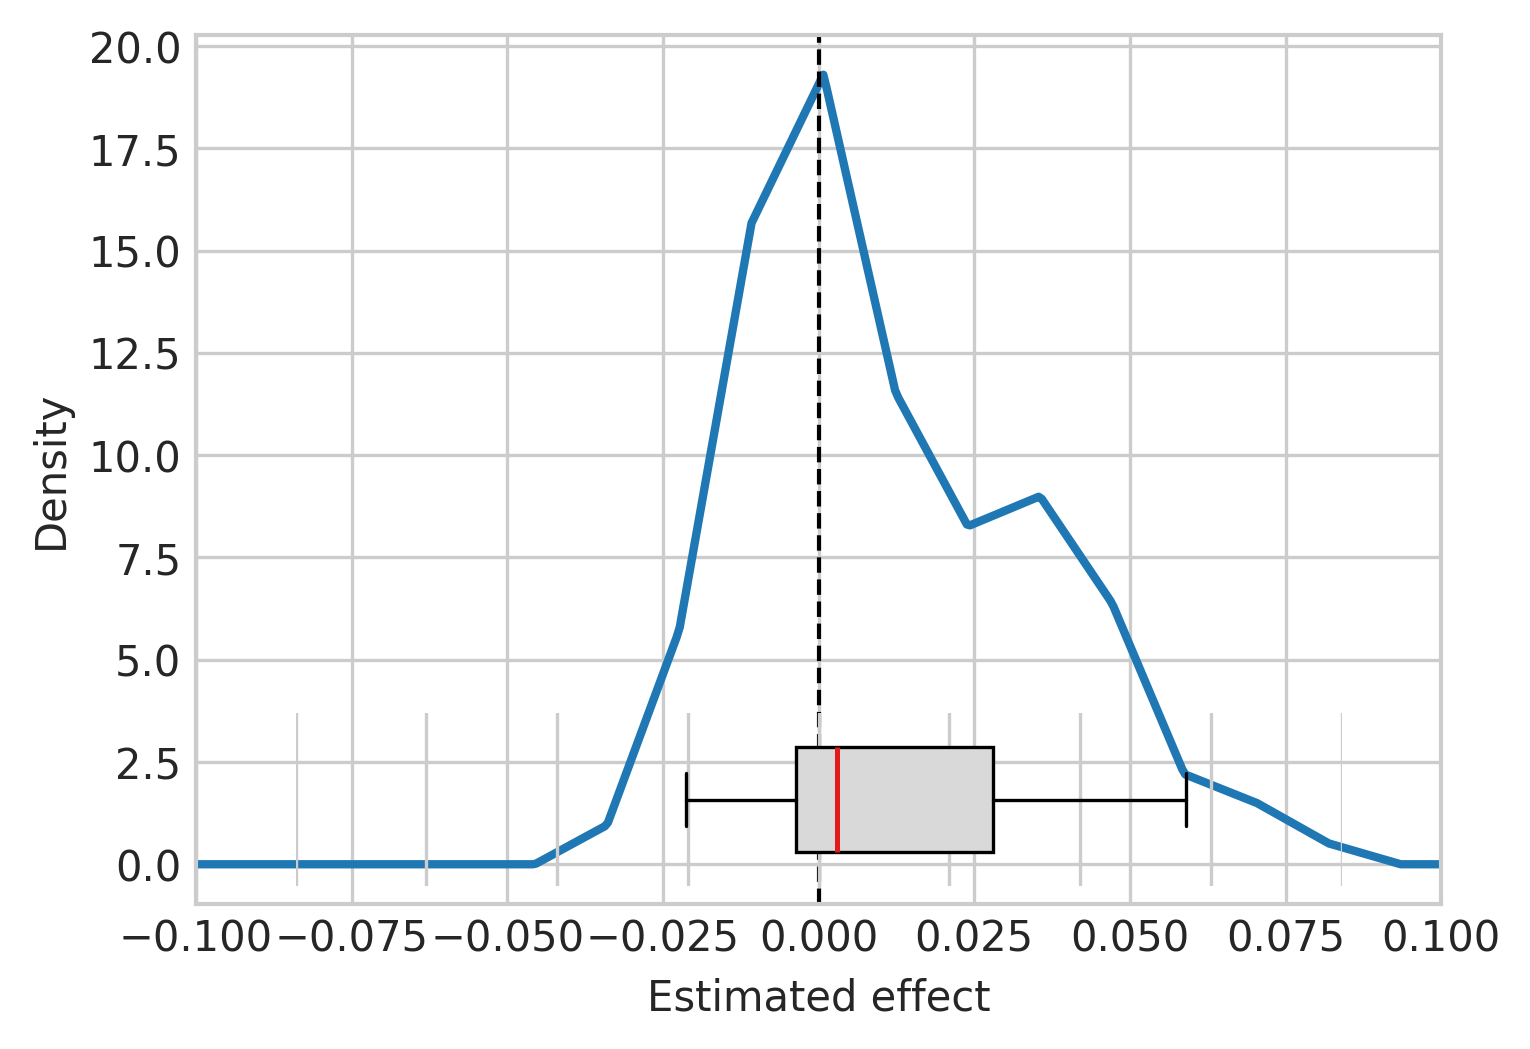
\includegraphics[width=\textwidth]{figure1_effect_unweighted.png}
    \caption{Unweighted}
\end{subfigure}
\hfill
\begin{subfigure}[b]{0.48\textwidth}
    \centering
    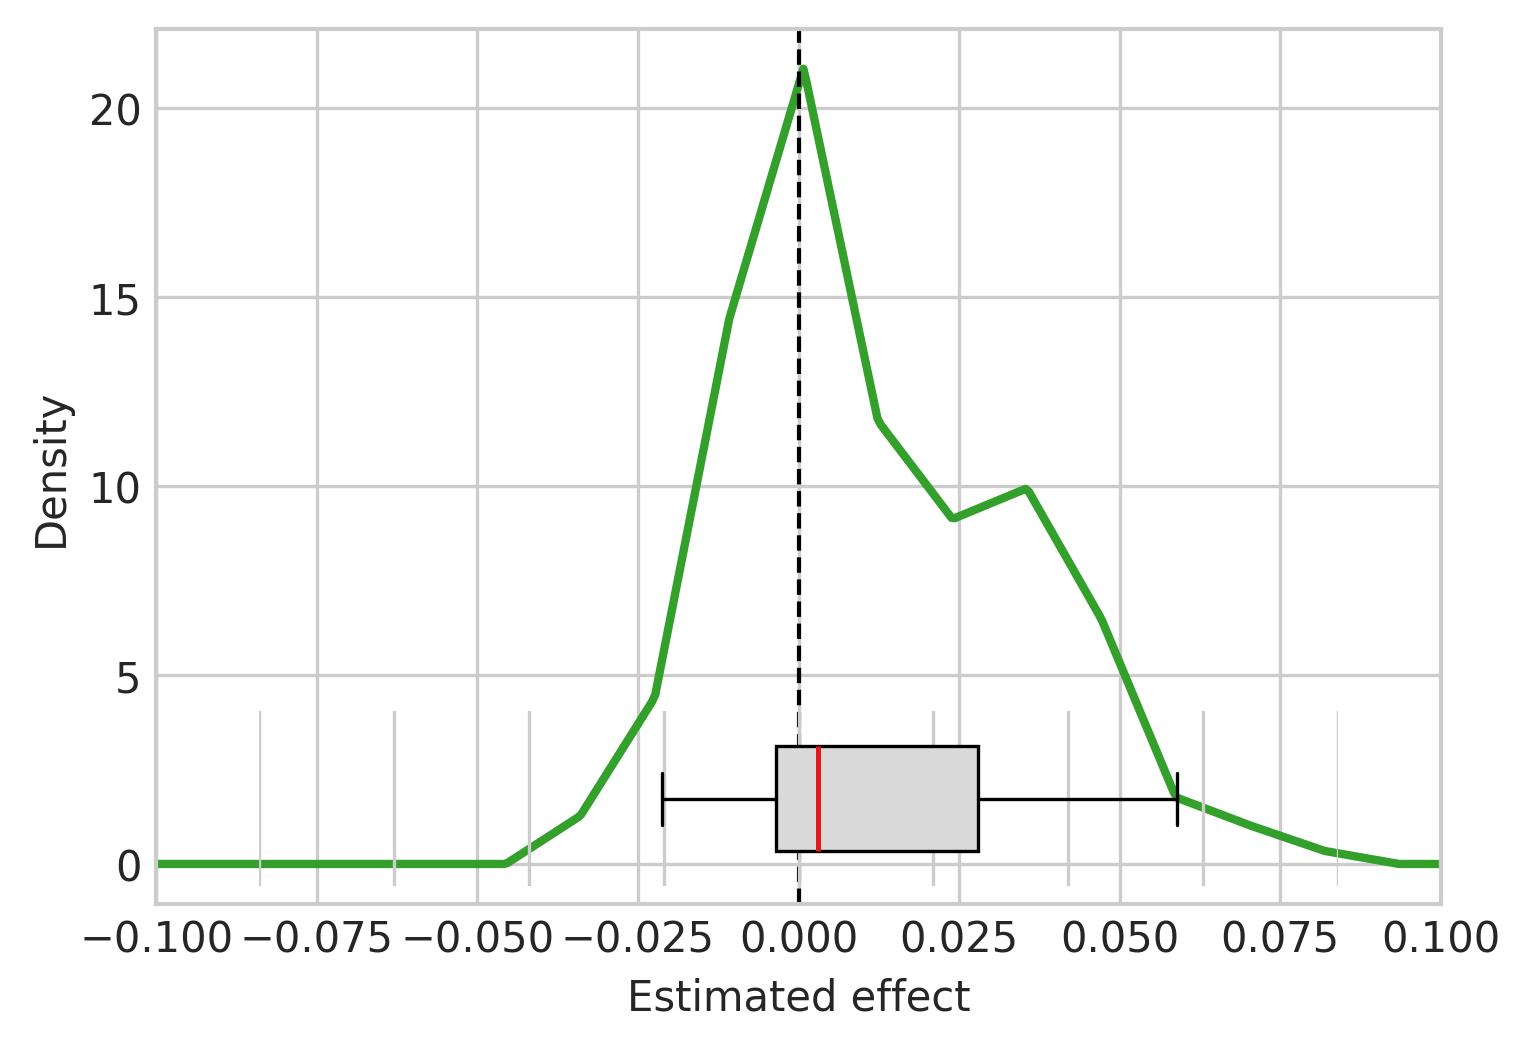
\includegraphics[width=\textwidth]{figure1_effect_weighted.png}
    \caption{Weighted by inverse SE}
\end{subfigure}
\caption{Distribution of reported effect sizes}
\caption*{\textbf{Notes:} Each panel shows an Epanechnikov kernel density of point estimates (Scott bandwidth). The box-and-whisker strip overlaid on the x-axis shows the median (red line), the interquartile range (box), and whiskers extending to the sample minimum and maximum. Inverse-SE weights use $1/\max(SE, q_{0.25})$, where $q_{0.25}$ is the 25th percentile of $SE$, to prevent a single near-zero standard error from dominating. For visual clarity, the x-axis is restricted to $[-0.1, 0.1]$, so tails beyond this range are not shown.}
\label{fig:effects}
\end{figure}

\begin{figure}[htbp]
\centering
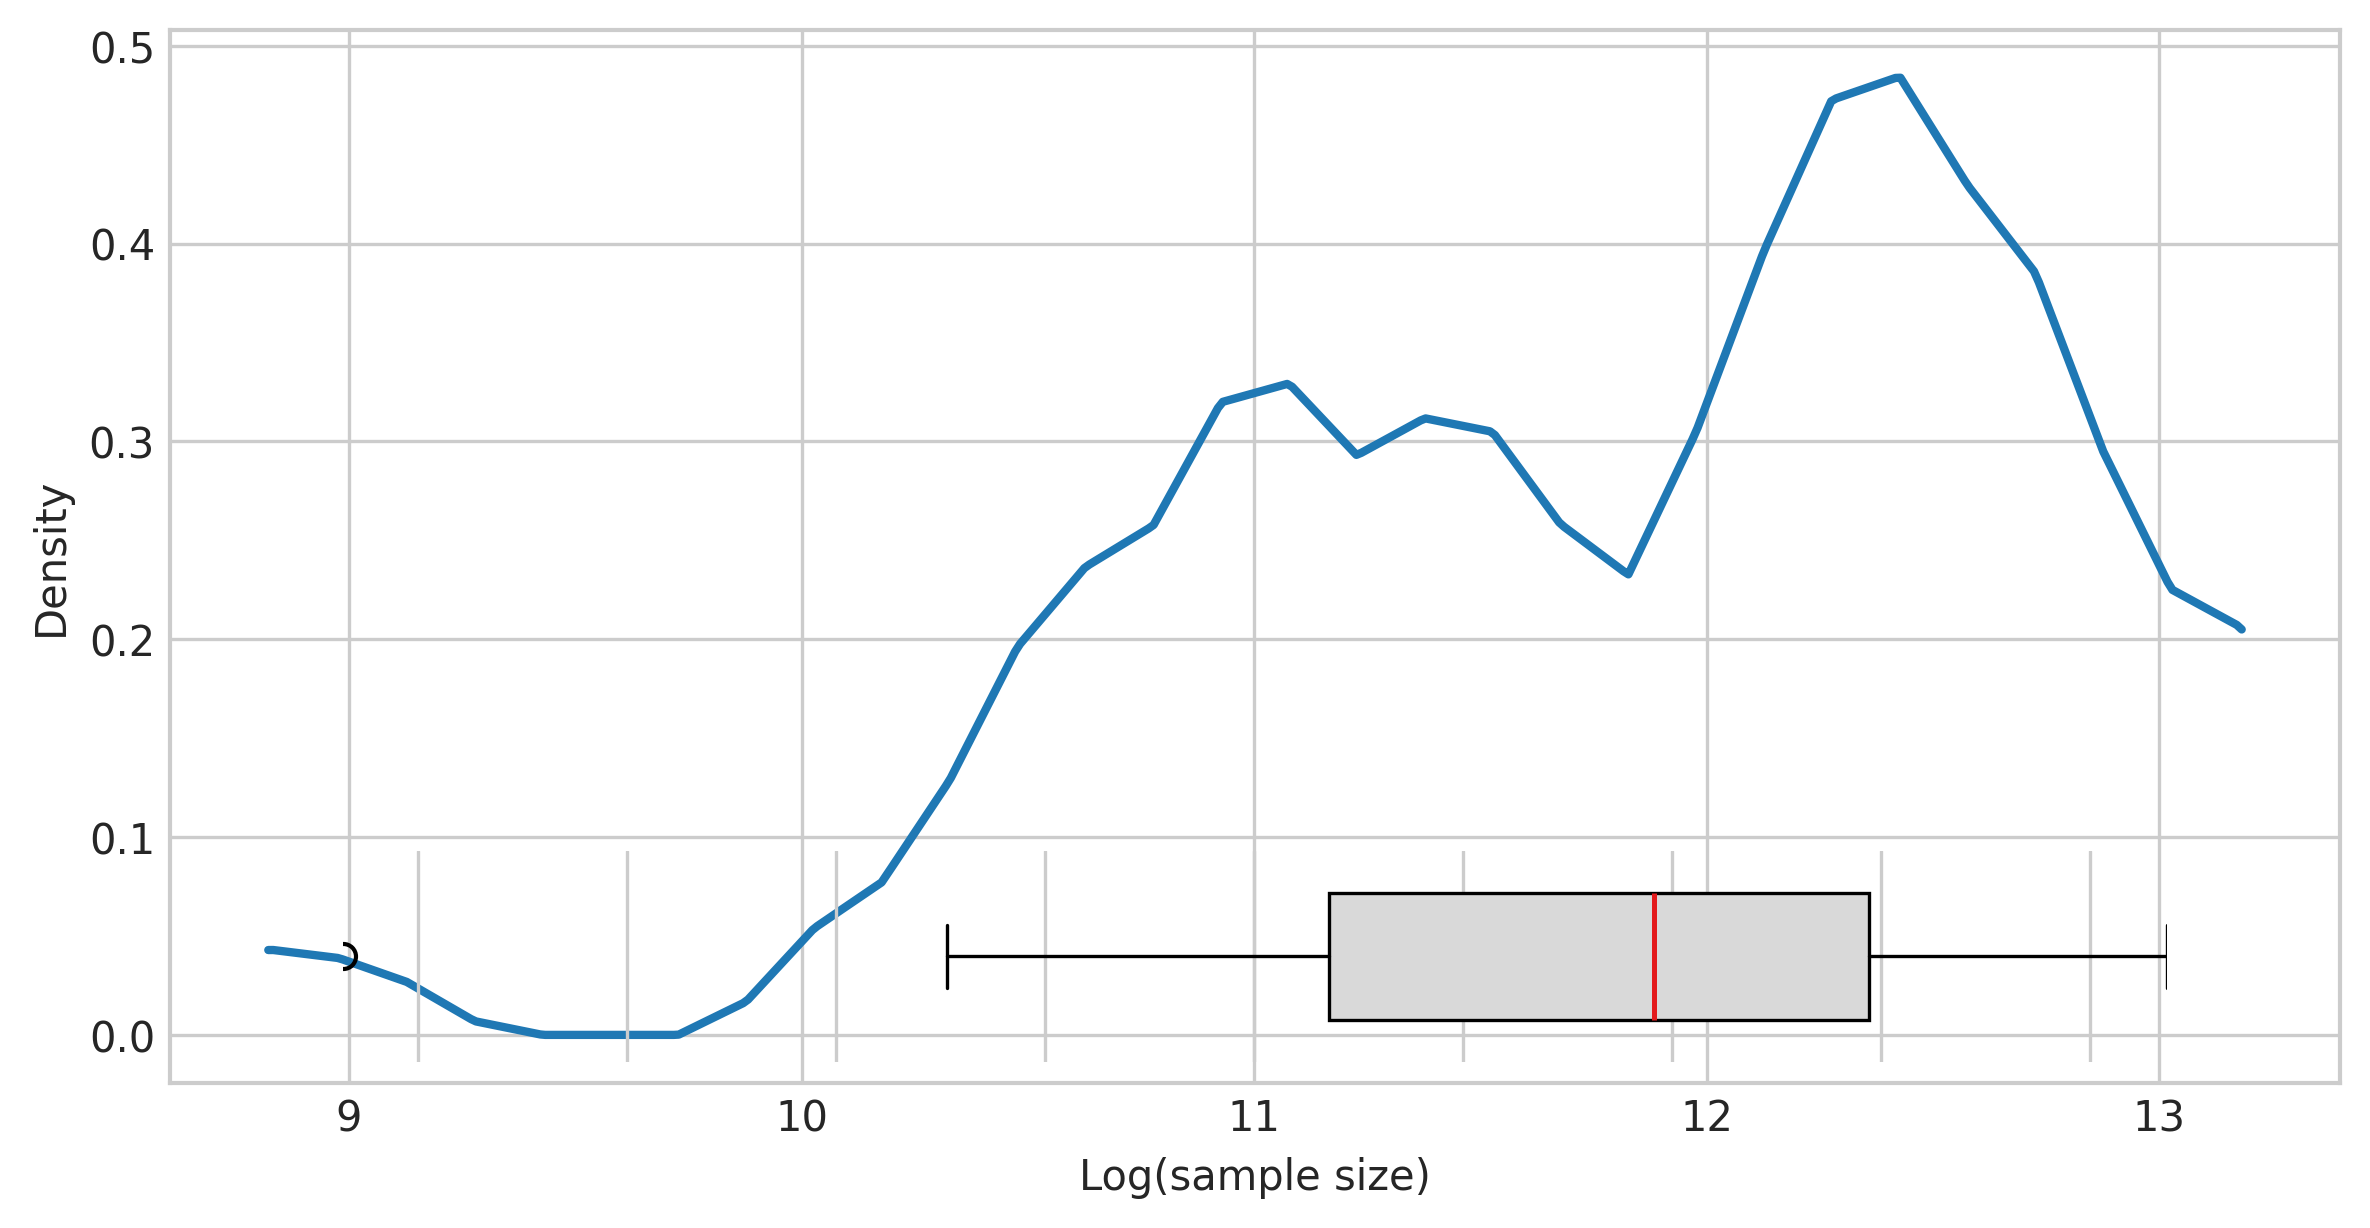
\includegraphics[width=\textwidth]{figure2_sample_size_distribution.png}
\caption{Distribution of sample sizes}
\caption*{\textbf{Notes:} The plot shows an Epanechnikov kernel density of $\log(\text{sample size})$ across specifications (Scott bandwidth). The box-and-whisker strip overlaid on the x-axis shows the median (red line), the interquartile range (box), and whiskers extending to the sample minimum and maximum. Differences arise from LLM choices about sample restrictions, cohort definitions, and treatment timing windows.}
\label{fig:samplesize}
\end{figure}

\begin{figure}[htbp]
\centering
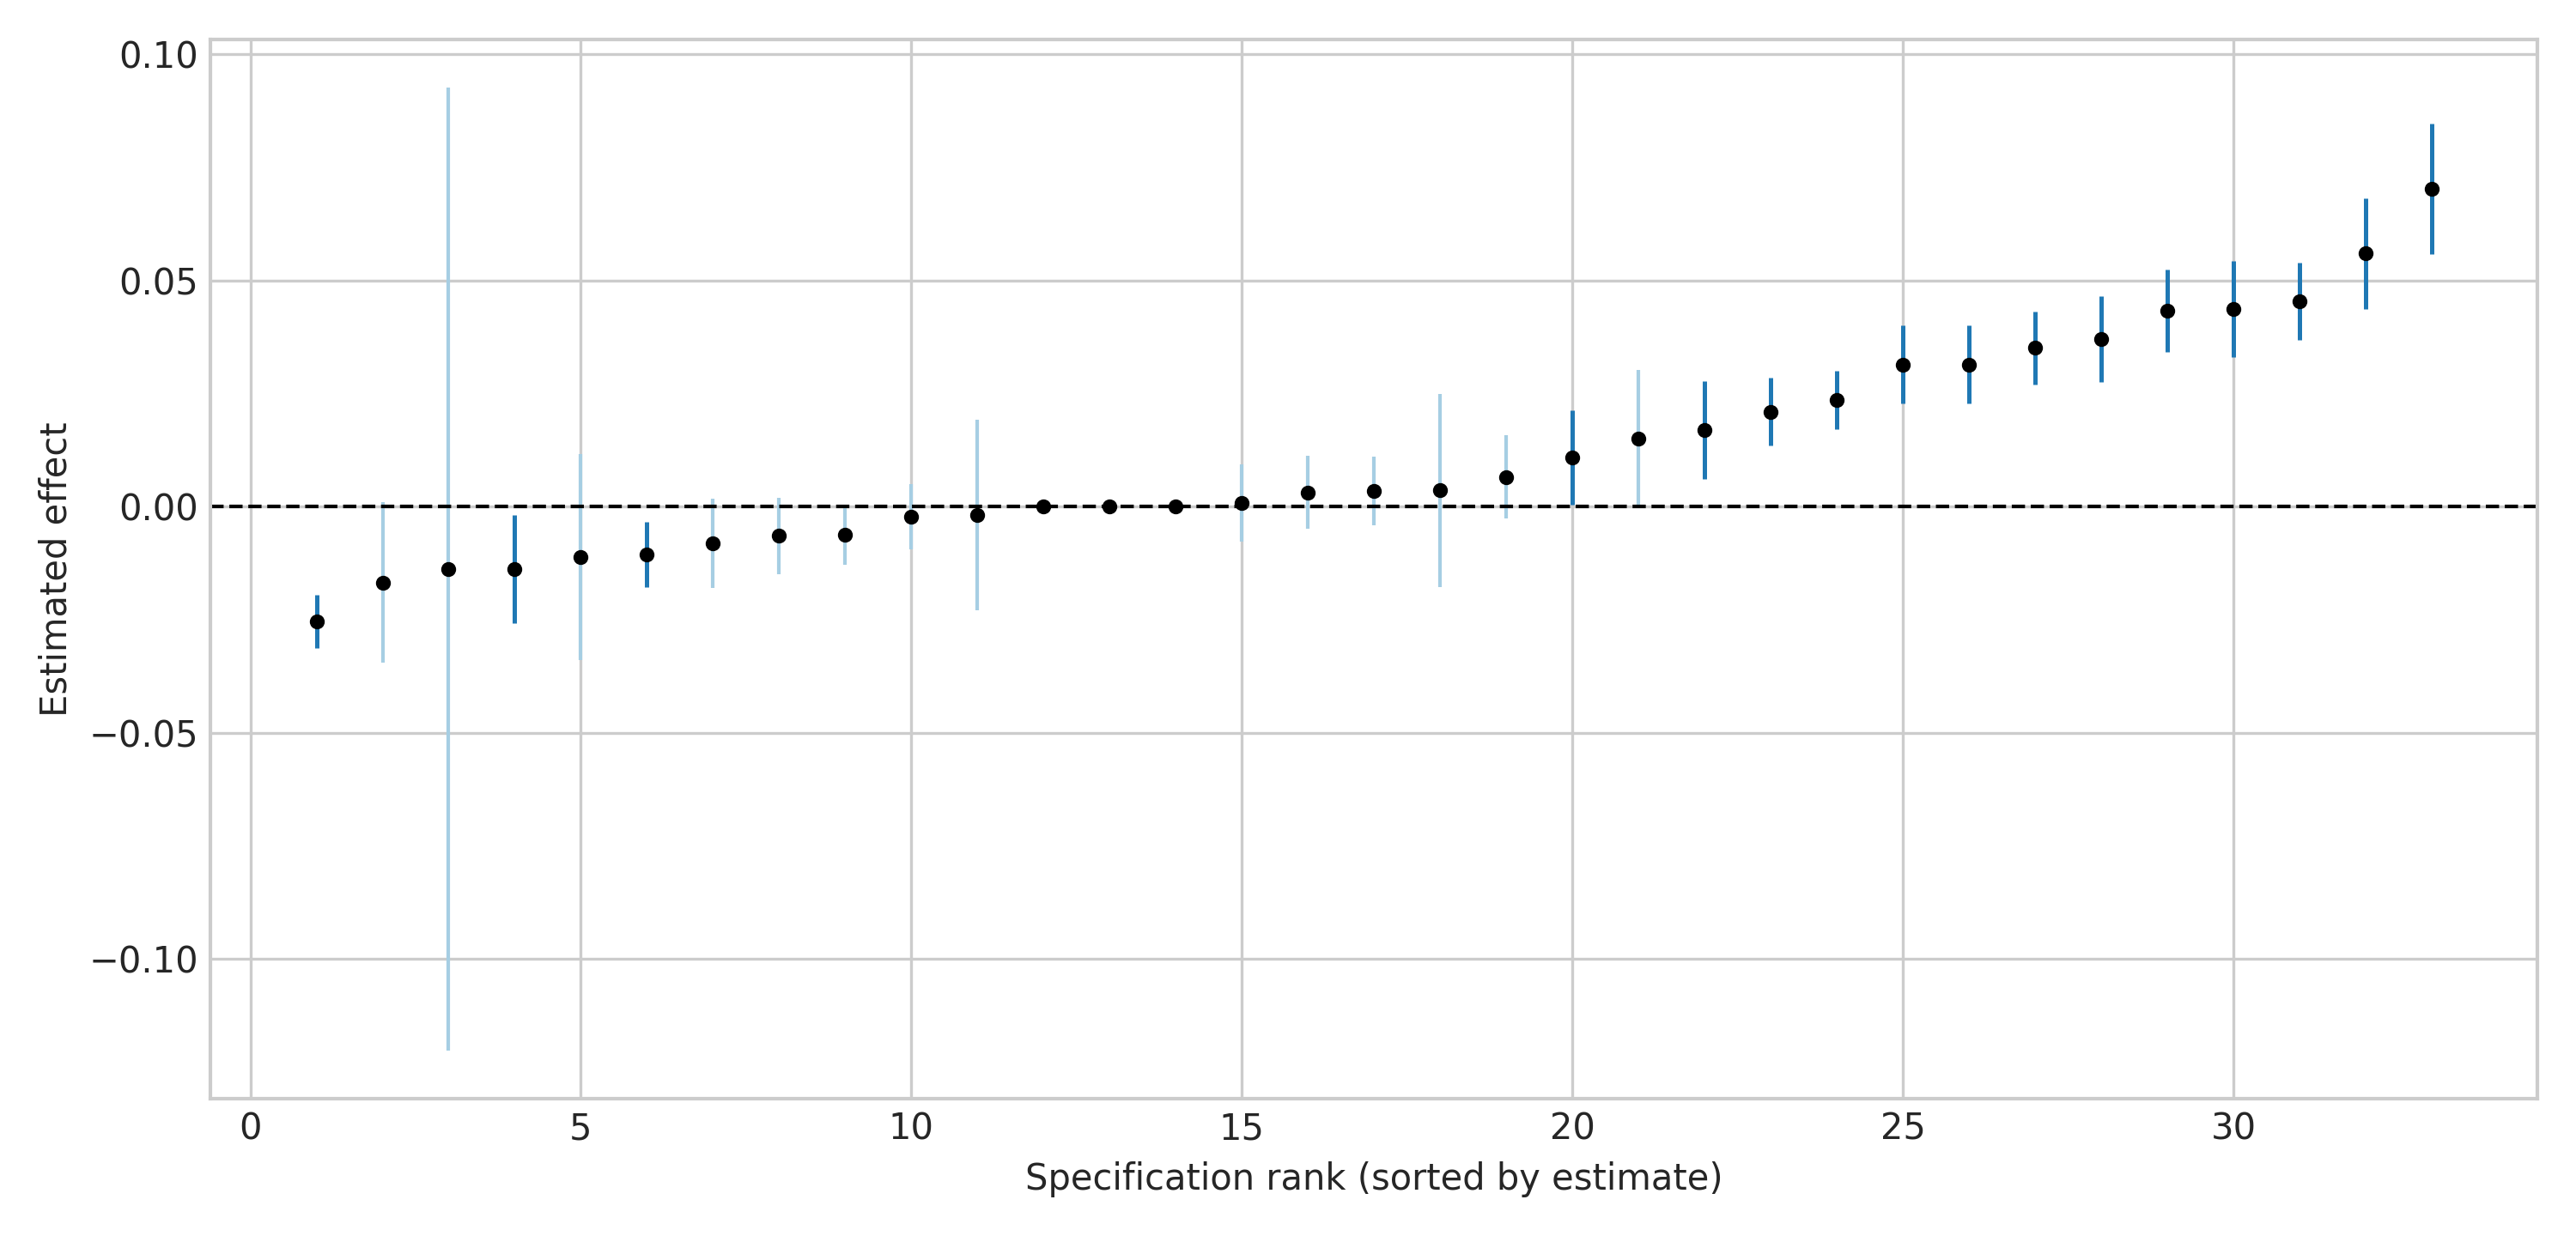
\includegraphics[width=\textwidth]{figure3_specification_curve.png}
\caption{Specification curve of DACA employment estimates}
\caption*{\textbf{Notes:} Each point corresponds to one specification, ordered by the point estimate from smallest to largest. Vertical bars show 95\% confidence intervals computed as $\hat{\beta} \pm 1.96 \times SE$. Dark blue intervals denote statistical significance at the 5\% level (confidence interval excludes zero). Light blue intervals denote non-significant estimates. For visual clarity, the figure is restricted to point estimates in $[-0.1, 0.15]$; specifications outside this range are omitted. No multiple-testing adjustment is applied; the figure is descriptive.}
\label{fig:speccurve}
\end{figure}

\begin{table}[htbp]
\centering
\caption{Shares of runs by estimation method, weighting, and variance adjustment}
\begin{tabular}{@{}l l r r@{}}
\toprule
Category & Choice & N & Share (\%) \\
\midrule
Estimation Method & OLS & 15 & 42.9 \\
 & Other & 4 & 11.4 \\
 & WLS & 16 & 45.7 \\
Sample Weighting & None & 17 & 48.6 \\
 & PERWT & 18 & 51.4 \\
SE Adjustment & Clustered (state) & 25 & 71.4 \\
 & None & 8 & 22.9 \\
 & Robust (HC) & 2 & 5.7 \\
\bottomrule
\end{tabular}
\caption*{\textbf{Notes:} The table reports the number and share of valid runs using each estimation method, sample-weighting choice, and standard-error adjustment. ``Clustered (state)'' indicates cluster-robust standard errors with clustering at the state level. ``Robust (HC)'' includes heteroskedasticity-consistent variance estimators when specified. ``Other'' groups any estimation or weighting choices not labeled as OLS/WLS or PERWT.}
\label{tab:methods}
\end{table}

\begin{table}[htbp]
\centering
\caption{Mean effects by functional form of control variables}
\begin{tabular}{@{}l l r r r@{}}
\toprule
Control Variable & Functional Form & N & Mean Effect & SD \\
\midrule
Age & Linear (AGE) & 17 & 0.006 & 0.061 \\
 & Quadratic (AGE + AGE\textasciicircum{}2) & 15 & 0.032 & 0.084 \\
 & Fixed Effects C(AGE) & 7 & 0.002 & 0.032 \\
 & Not included & 47 & 0.007 & 0.096 \\
Sex & Fixed Effects C(SEX) & 23 & 0.010 & 0.051 \\
 & Not included & 63 & 0.011 & 0.093 \\
Education & Fixed Effects C(EDUC) & 14 & 0.021 & 0.023 \\
 & Not included & 72 & 0.009 & 0.091 \\
Year FE & Included & 52 & 0.022 & 0.083 \\
 & Not included & 34 & -0.007 & 0.083 \\
State FE & Included & 47 & 0.023 & 0.086 \\
 & Not included & 39 & -0.004 & 0.079 \\
\bottomrule
\end{tabular}
\caption*{\textbf{Notes:} For each control variable, the table reports the mean and standard deviation of point estimates among specifications using that functional form. ``Fixed Effects'' indicates categorical controls (e.g., $C(\text{EDUC})$). ``Not included'' indicates that the control was omitted entirely from the specification.}
\label{tab:controls}
\end{table}

\begin{table}[htbp]
\centering
\caption{Summary statistics by LLM provider}
\begin{tabular}{@{}l r r r r@{}}
\toprule
Statistic & GPT 5.1 Codex Mini & OpenAI Codex CLI & Mistral Devstral Medium & Google Gemini 3 Flash \\
\midrule
N & 38 & 18 & 20 & 10 \\
Mean point\_est & -0.001 & 0.020 & 0.021 & 0.017 \\
SD point\_est & 0.079 & 0.020 & 0.133 & 0.031 \\
IQR point\_est & 0.079 & 0.033 & 0.051 & 0.049 \\
\bottomrule
\end{tabular}
\caption*{\textbf{Notes:} Columns correspond to the Phase 1 LLM provider that generated each specification. Statistics are computed on the same filtered sample as Table~\ref{tab:summary}. The IQR is the 75th minus 25th percentile of point estimates within each provider.}
\label{tab:providers}
\end{table}

\section{Discussion}
The specification curve and distributional summaries highlight substantial researcher-induced variation in estimated DACA employment effects, even when all runs draw from the same underlying data. Differences in functional forms, fixed effects, weighting, and variance adjustments account for meaningful shifts in average estimates. Weighted densities place greater emphasis on higher-precision runs, which helps distinguish variation driven by specification choices from variation driven by noisier samples.

This Phase 4 meta-analysis provides a transparent, reproducible pipeline for quantifying researcher-choice variation. Because each LLM run produces an explicit model line and a concrete implementation in Phase 2, the resulting distribution of estimates can be traced directly back to specification features (e.g., functional form of age, presence of state or year fixed effects, or sample restrictions). Compared with the I4R ``Task 1'' setting, the LLM replications deliver a scalable way to map the specification space while preserving interpretability of each estimated effect. Future phases will extend the analysis to constrained tasks and alternative prompting strategies to better calibrate LLM-induced variation to human researcher heterogeneity.

\end{document}
